\documentclass{article}
\usepackage{graphicx}
\usepackage[utf8]{inputenc}
\usepackage{geometry}
\usepackage{float}
\geometry{a4paper, margin=1in}

\title{Relatório de Alinhamento de Sequências (Smith-Waterman)}
\author{Bioinformática}
\date{\today}

\begin{document}

\maketitle

\section{Matriz de Scores (Todos contra Todos)}
Abaixo apresentamos a matriz de scores resultante da comparação de todas as sequências entre si. Esta tabela exibe a pontuação máxima obtida no alinhamento local entre cada par de sequências.

\begin{figure}[H]
    \centering
    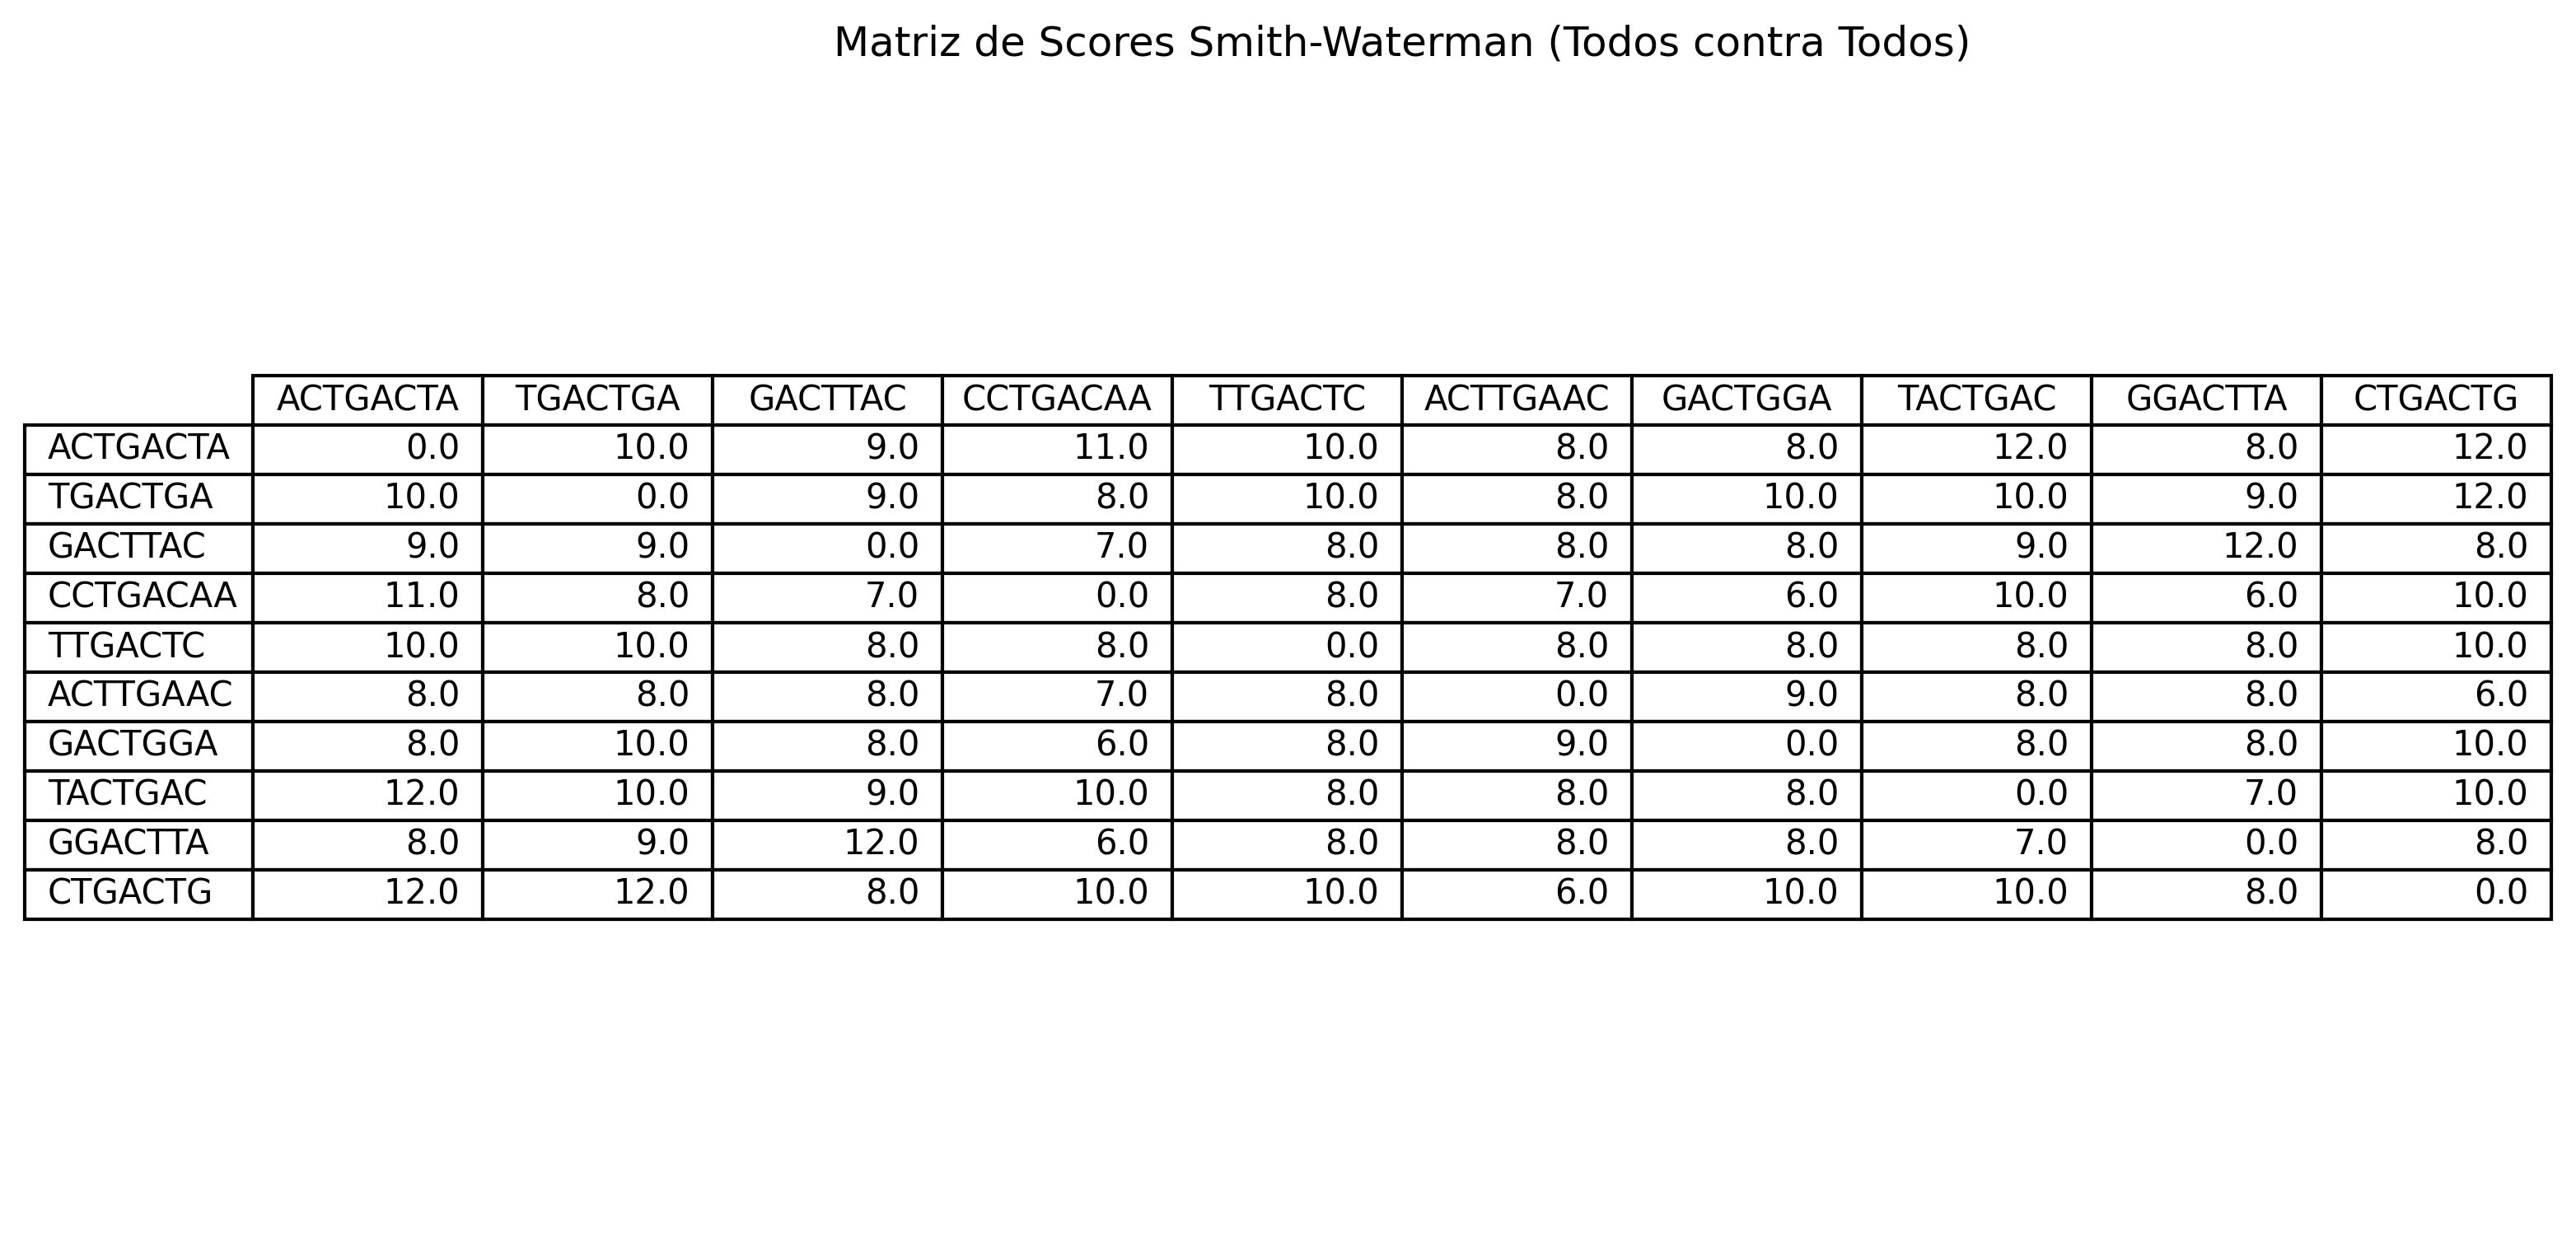
\includegraphics[width=0.9\textwidth]{tabela_comparacao.png}
    \caption{Matriz de Scores Smith-Waterman}
\end{figure}

\newpage

\section{Matriz de Melhores Alinhamentos Locais}
Nesta seção, visualizamos os alinhamentos literais (bases alinhadas) correspondentes aos scores máximos obtidos. Devido ao tamanho, a imagem foi ajustada para melhor visualização.

\begin{figure}[H]
    \centering
    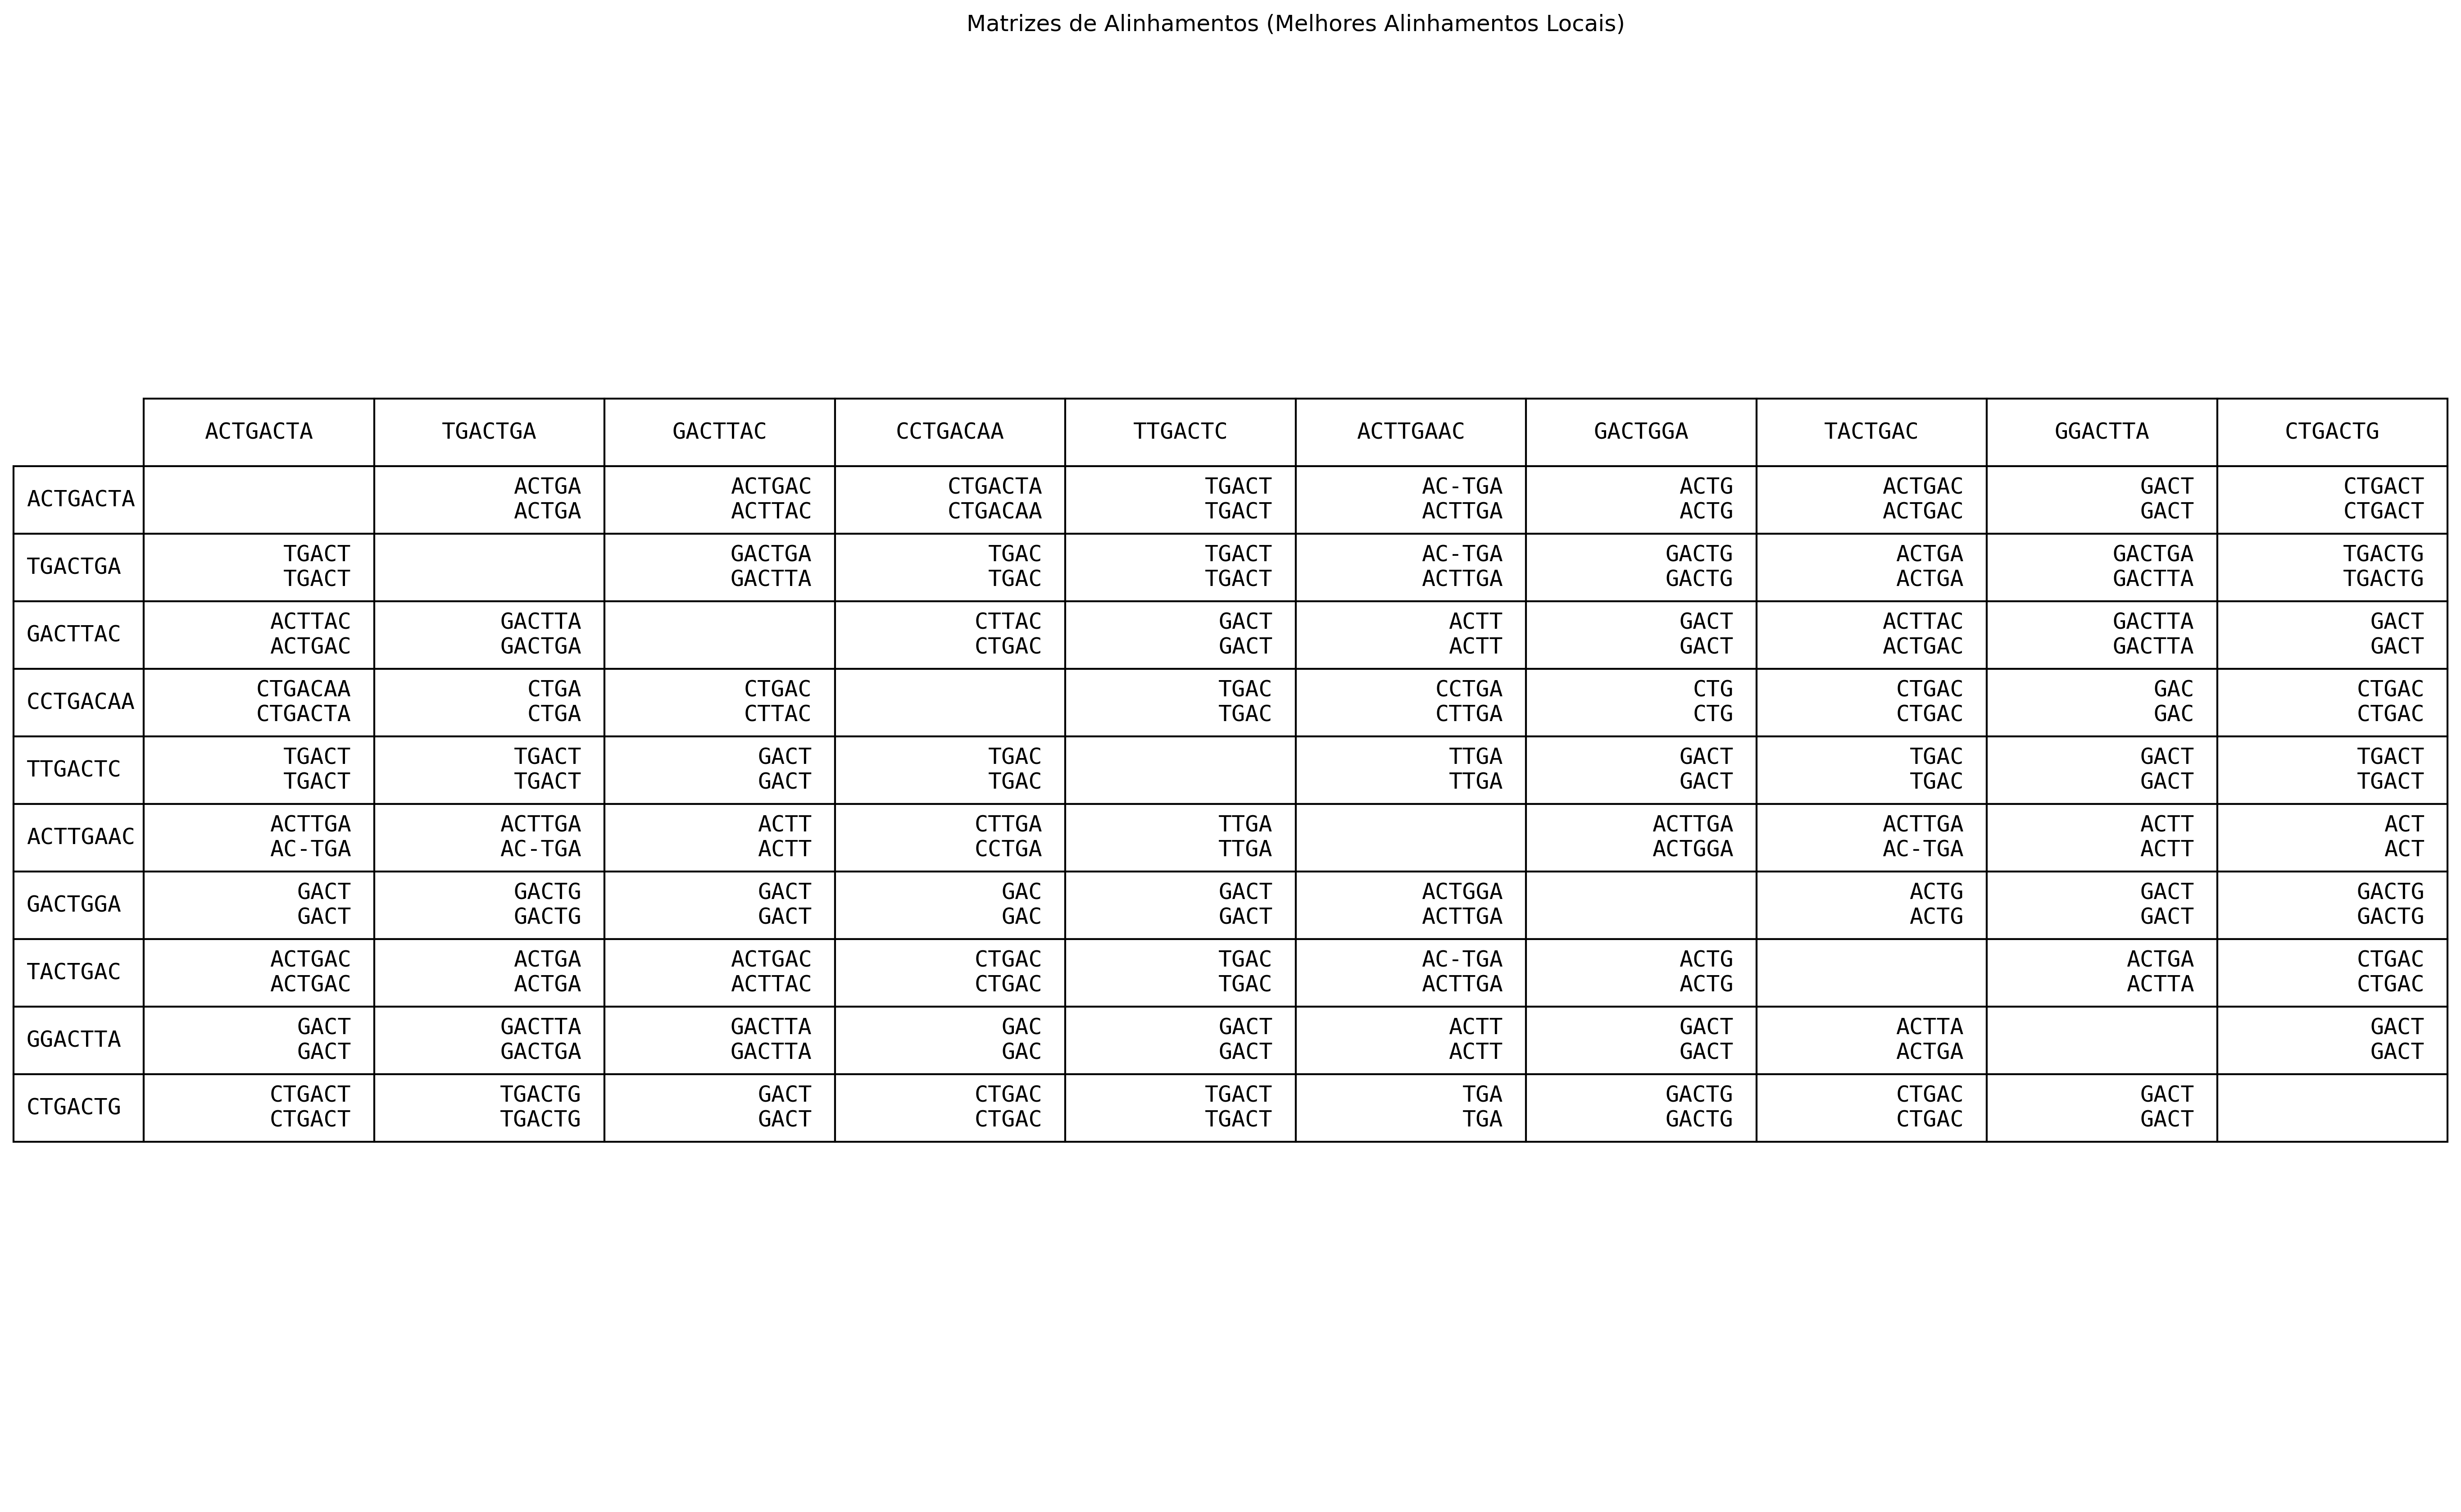
\includegraphics[width=0.95\textwidth]{tabela_alinhamentos.png}
    \caption{Tabela com os alinhamentos gerados}
\end{figure}

\section{Top 2 Melhores Alinhamentos}
Destaque para os dois melhores alinhamentos encontrados em todo o conjunto de dados (excluindo a comparação de uma sequência com ela mesma).

\begin{figure}[H]
    \centering
    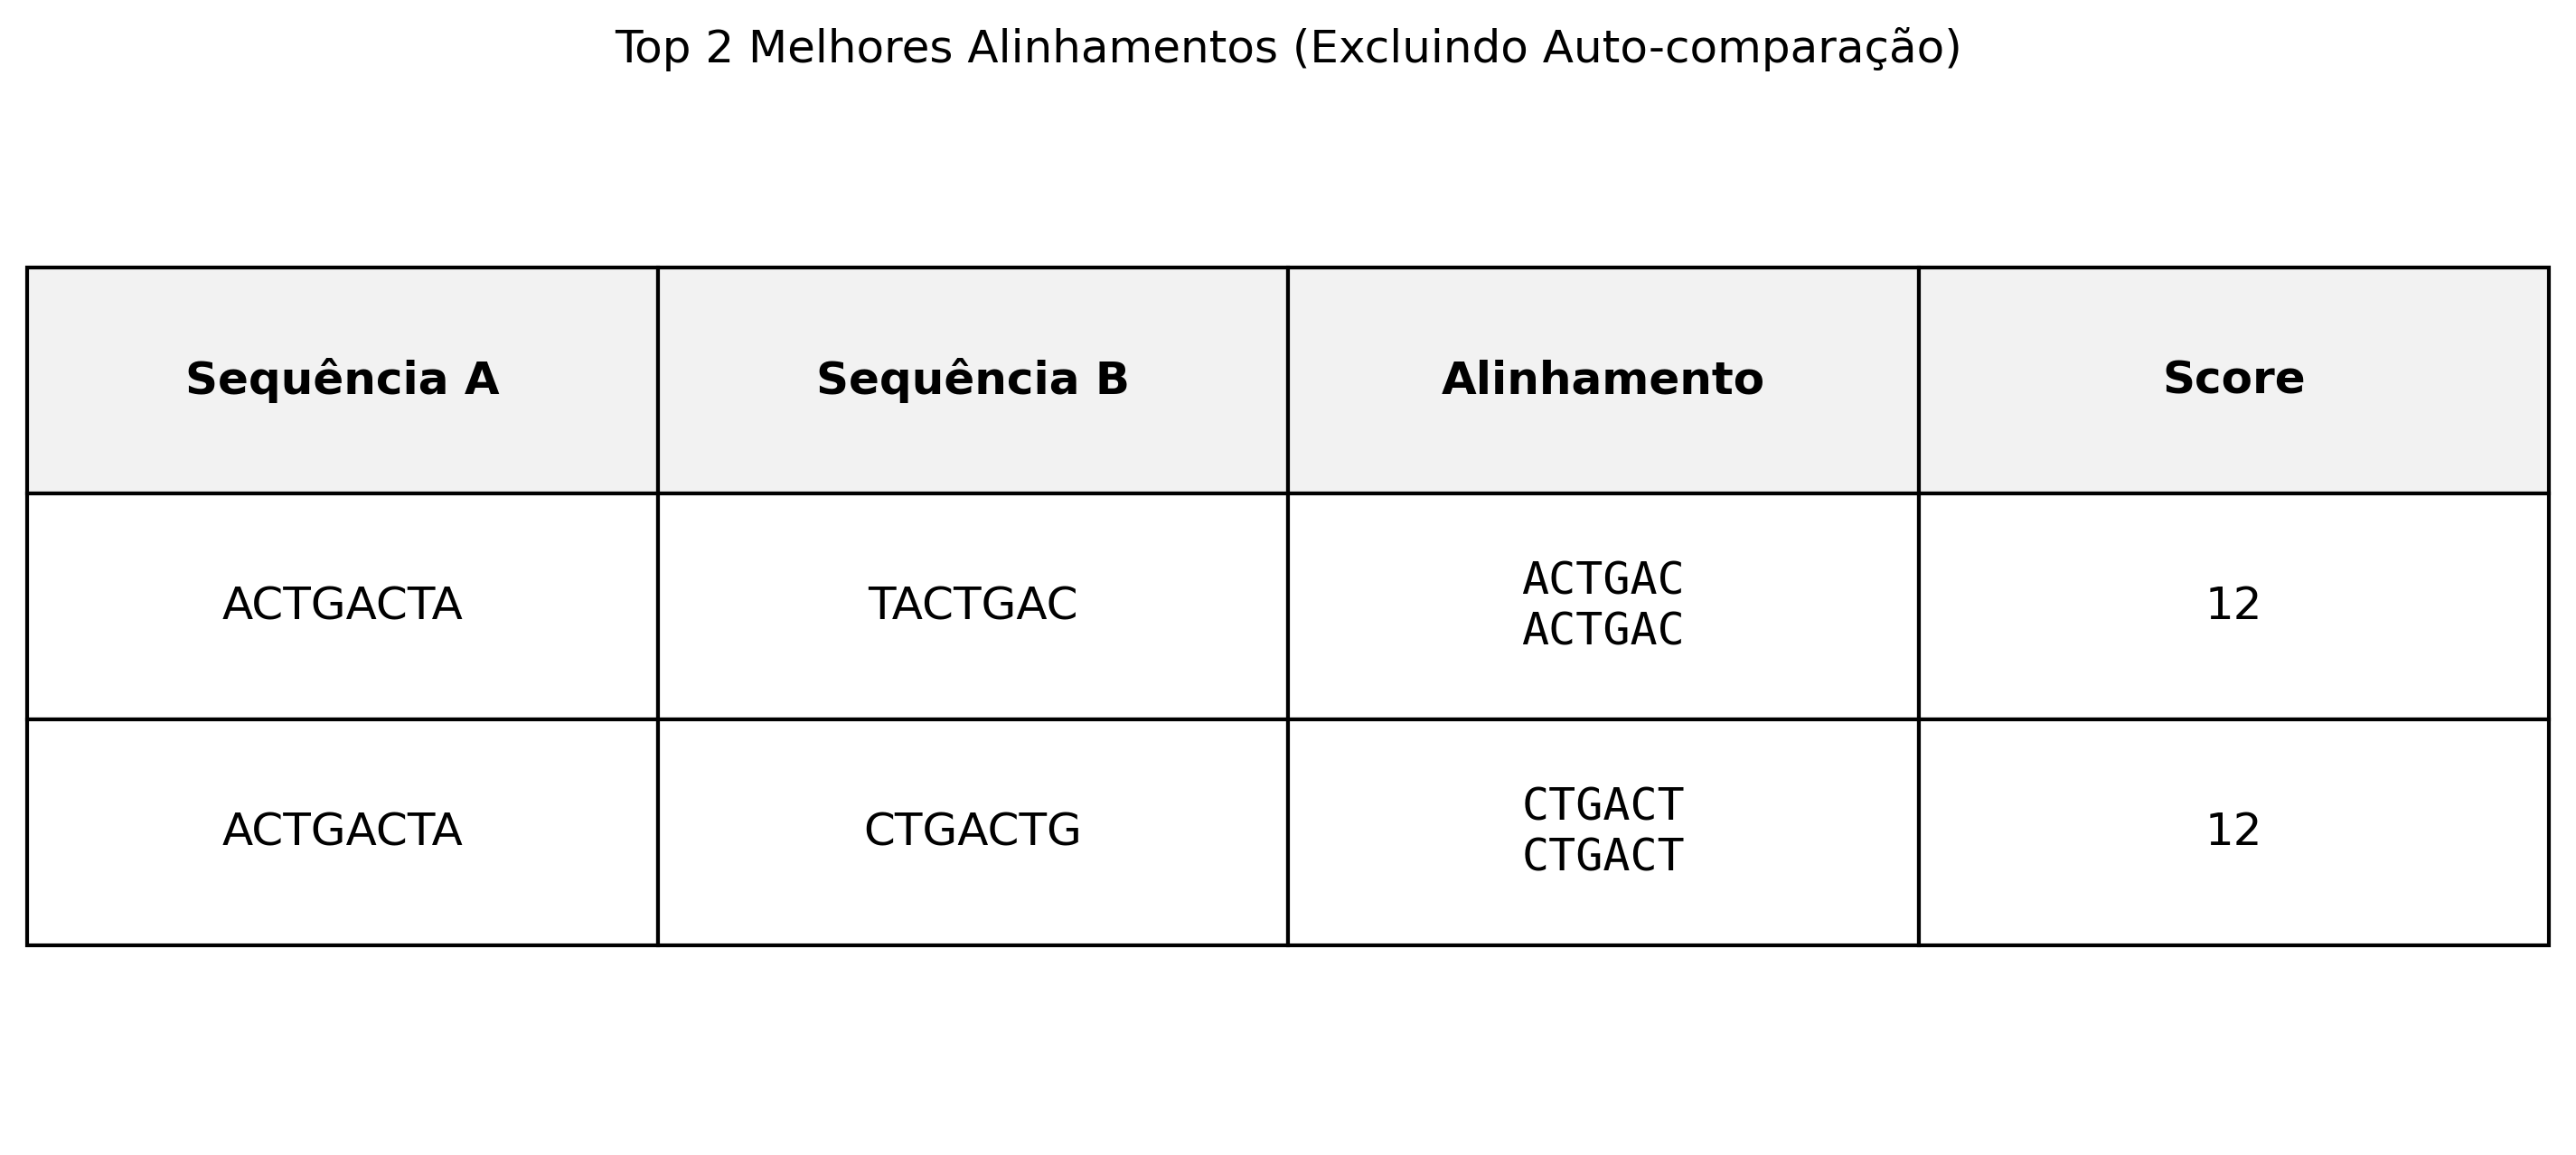
\includegraphics[width=0.9\textwidth]{tabela_top2.png}
    \caption{Ranking dos Top 2 Alinhamentos}
\end{figure}

\end{document}
